%
% ======================================================================

\RequirePackage{docswitch}
% \flag is set by the user, through the makefile:
%    make note
%    make apj
% etc.
\setjournal{\flag}

\documentclass[\docopts]{\docclass}

% You could also define the document class directly
%\documentclass[]{emulateapj}

% Custom commands from LSST DESC, see texmf/styles/lsstdesc_macros.sty
\usepackage{lsstdesc_macros}
\usepackage{graphicx}
\graphicspath{{./}{./figures/}}
\bibliographystyle{apj}
% \usepackage{subcaption}
% \captionsetup{compatibility=false}
% Add your own macros here:
\usepackage{etoolbox}
%\usepackage{stackengine}
\setcounter{secnumdepth}{4}
\usepackage{csvsimple}
% \usepackage{hyperref}
% \usepackage{adjustbox}
\usepackage{xspace}
\usepackage{numprint}

\def\aapr{A\&A~Reviews}
\def\SLRealizer{\texttt{SLRealizer}\xspace}
\def\Object{\texttt{Object}\xspace}
\def\Source{\texttt{Source}\xspace}
\def\DIAObject{\texttt{DIAObject}\xspace}
\def\DIASource{\texttt{DIASource}\xspace}
\def\GalSim{\texttt{GalSim}\xspace}
\def\sklearn{\texttt{scikit-learn}\xspace}

% ======================================================================

\begin{document}

\title{\SLRealizer: LSST Catalog-level Realization of Gravitationally-lensed Quasars }

\maketitlepre

\begin{abstract}

The scale of the LSST dataset will be such that, when considering the
problem of finding lensed quasars, we should anticipate extracting as
much information out of the the catalogs as possible before turning to
the pixel-level data. In this work we explore the use of simple, low
multiplicity Gaussian mixture models for realizing gravitational lens
systems in LSST catalog space, to enable both large-scale data
emulation and fast initial lens-or-not classification. We demonstrate
the generation of toy \Source and \Object catalogs, and carry out a
simple machine learning classification using them.

\end{abstract}

% Keywords are ignored in the LSST DESC Note style:
\dockeys{methods: statistical, cosmology: gravitational lenses}

\maketitlepost

% ----------------------------------------------------------------------

\section{Introduction}
\label{sec:intro}

% The Large Synoptic Survey Telescope (LSST), a wide-field survey telescope with the diameter
% of 8.4m, will start running in Chile in 2020 \cite{LSST_overall}. This
% telescope has a 3.5 $deg$ of field of view, would cover around 30000
% $\textit{deg}^2$ in the sky, and uses $u$, $g$, $r$, $i$, $z$, and $y$
% filters \cite{LSSTScienceBookv2}. The telescope will give an extensive
% amount of astronomical data that could be used for the study of Solar
% System, Extragalactic structures, near-Earth asteroids, radiant radio
% sources, Dark Matter, and Dark Energy \cite{LSSTScienceBookv2}.

We anticipate being able to detect around 8000 strongly lensed quasar
systems, that will provide useful information on lens mass distributions
and cosmological time delay distances \citep{TM16,Twinkles}.
% Time delay could be used to infer cosmological parameters
% \cite{Treu2010} which describes the state of the universe.
Finding these lensed systems among the billions of objects detected and
measured by LSST \citep{LSSTScienceBookv2} is a key challenge.
Pixel-level searches \citep[e.g.\ ]{RINGFINDER} may be unfeasible,
unless the targets are efficiently pre-selected.  We can imagine doing
an initial lens classification on {\it catalog-level} data using machine
learning techniques, in order to make this pre-selection.

Machine learning to detect gravitational lensed systems is an active
area of research, with most of the focus to data being on galaxy-galaxy
``Einstein Ring'' systems, where  morphological classification using
Convolutional Neural Networks (CNN) should be effective
\citep{convolution_neural_network}. Early experiments show some
promising results \citep{LensExtractor,CMUDeepLens,JacobsEtal2017}. The LSST
catalog can be thought of as a database of pre-extracted low-level image
features, which can be used as inputs to machine learning techniques.
How much lensing information do these features contain? Do we need to
form higher-level features (somehow) before feeding them to a machine
classifier? How can we best train a machine to classify the LSST
\Object's as lenses or nots, without requesting the images?

To answer these questions, we construct a mock LSST dataset, emulating
the action of the LSST data management software stack in generating the
data release catalog. Our simple emulator is called \SLRealizer: we
explain the assumptions it encodes in \autoref{sec:method} below, and
present a small toy emulated LSST dataset made with \SLRealizer in
\autoref{sec:data}. We then carry out a simple demonstration machine
classification, training and testing the machine on a our toy \Object
table, in \autoref{sec:ml}. We draw some conclusions about future work
in \autoref{sec:conclusions}.

% ----------------------------------------------------------------------

\section{\SLRealizer}
\label{sec:method}

\subsection{Model assumptions}
\label{subsec:model}

\SLRealizer takes as input an extragalactic catalog of mock lensed
quasar systems, and emulates the LSST data release catalog measurements
of those lenses. It's assumptions are that the \Object's and \Source's
in the catalog tables can be simply represented as mixtures of
Gaussians, and measurements of them derived from those Gaussian
mixtures.

Specifically, we assume that a lensed quasar system is composed of 2 or
4 point sources (for doubles and quads respectively), plus a lens
galaxy that can be represented with an elliptically-symmetric Gaussian
surface brightness distribution. The seeing FWHM in each visit is used
to define a circularly-symmetric Gaussian PSF.

\SLRealizer models the action of the LSST DM stack deblender as
returning a single \Object for each galaxy-scale lensed quasar system.
Its ``null deblender'' yields predictions of the flux, position, size
and ellipticity of each measured \Source calculated by realizing the
surface brightness of the PSF-convolved system on a pixelated
``pseudo-image'' grid, and then numerically integrating this image to
obtain its zeroth, first and second moments. We use the python \GalSim
package to carry out the pseudo-image manipulations, and choose a pixel
scale of 0.2~arcseconds (the same as the LSST detectors).

Gaussian noise is added to each measurement, based on a simple error
model.

The \Object table is then emulated by simply averaging the available
\Source flux, position, size and ellipticity measurements in each
filter.


\subsection{Emulator Inputs}
\label{subsec:inputs}

Twinkles, a simulated LSST sky with observed with six filters for ten
years, used ten years of mock observation history from the LSST
Project's baseline cadence simulation, \texttt{minion\_1016}. We use
this history file to define an MJD date, filter, seeing FWHM and 5-sigma
limiting depth for each visit in the history, and select just the first
three years of observations, which yields 263 observation epochs.

\begin{table}[!h]
\csvautotabular{../../data/twinkles_observation_history_head.csv}
%https://texblog.org/2012/05/30/generate-latex-tables-from-csv-files-excel/ %bug
% PJM: The following doesn't work:
% \csvreader[head to column names, tabular=lllll,
% table head=\toprule, \bfseries obsHistID & \bfseries expMJD & \bfseries filter & \bfseries FHWMeff & \bfseries fiveSigmaDepth \\ \midrule,
% table foot=\bottomrule,
% filter test=\ifnumless{\obshistid}{187546}]%
% {../../data/twinkles_observation_history.csv}{}{%
% \thecsvrow & \obshistid & \expmjd & \filter & \fwhmeff & \fiveSigmaDepth }
%
\caption{A few entries of the Twinkles mock observation history data.
The full dataset can be accessed
\href{https://github.com/LSSTDESC/SLRealizer/blob/master/data/twinkles_observation_history.csv}{here}.}
\end{table}

We use the OM10 mock lens catalog \citep{OM10} to define the properties
of the lens galaxy and lensed quasar images. We selected 2234 LSST-like
systems by querying with a magnitude cut of 22.5. Colors were computed
using the \href{https://github.com/drphilmarshall/OM10}{\texttt{OM10}} package, which makes use of the \href{https://github.com/tcollett/LensPop}{\texttt{LensPop}}
code \citep{LensPop} for estimating galaxy and quasar colors.

\begin{figure}
    \centering
    \begin{minipage}{0.48\linewidth}
        \centering
        
\includegraphics[width=\linewidth]{beforenulldeblend.png}
    \end{minipage}\hfill
    \begin{minipage}{0.48\linewidth}
        \centering
        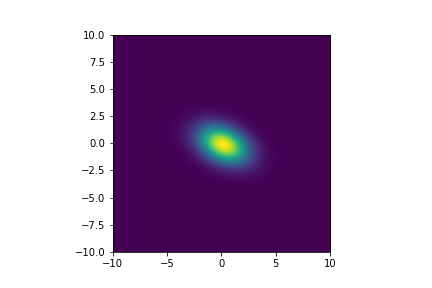
\includegraphics[width=\linewidth]{afternulldeblend.png}
    \end{minipage}
    \caption{Example null-deblending in OM10 lens system 4898214. Image
    axes show offsets from the  center of the lensed system in arcsec.
    Left: Realization of the lens system with zero-width PSF. The
    brightest source is the lensing galaxy, and there are two dimmer
    quasar images near the galaxy. There is only one quasar image that
    is obvious; this makes the blended object appear elliptical. Right:
    Realization of the lens system with realistic PSF. All the
    components of the system appear blended together. The color bar
    shows rescaled surface brightness: overall, flux is conserved
    between the two images.}
    \label{fig:null-deblend}
\end{figure}

% ----------------------------------------------------------------------

\section{Results: Toy Emulated LSST Data}
\label{sec:data}

A snippet from our toy \Source catalog is shown below, in
\autoref{tab:source}. As you can see, for now we have not calculated the positions (RA and DEC). The full catalog has 473596 rows, corresponding to approximately 212 observations of 2234 lenses.

\autoref{tab:object} shows an excerpt from our toy \Object catalog. The full \Object catalog has 2234 rows.


%%%%%%%%%%%%%%%%%%%%%%%%%%%%%%%%%%%%%%%%%%%
\begin{table}[!h]
\centering
\begin{tabular}{|l|l|l|l|l|l|l|l|l|l|l|}
\hline
lensid   & MJD          & filter & RA & RA\_err & DEC & DEC\_err & x              & x\_com\_err & y               & y\_com\_err \\ \hline
710960   & 59823.286523 & g      & 0  & 0       & 0   & 0        & 2.1350  & 0           & 1.2151 & 0			\\
17432684 & 59823.286523 & g      & 0  & 0       & 0   & 0        & 0.1226 & 0           & 0.7593  & 0           \\
50310149 & 59823.286523 & g      & 0  & 0       & 0   & 0        & 0.2527 & 0           & 0.4665  & 0           \\
52812164 & 59823.286523 & g      & 0  & 0       & 0   & 0        & 0.3874 & 0           & -0.3413 & 0          \\ \hline
\end{tabular}
\begin{tabular}{|l|l|l|l|l|l|l|l|l|l|}
\hline
flux          & flux\_err       & size          & size\_err & e1               & e2                & e               & phi             & psf\_sigma & sky       \\ \hline
21.9127 & 0.03549 & 1.4501 & 0         & 0.2386    & 0.3360    & 0.4121  & 0.4766  & 1.093153   & 24.377204 \\
18.2072 & 0.03549& 1.1802  & 0         & -0.0550 & -0.004712  & 0.05525 & 0.04270 & 1.093153   & 24.377204 \\
5.9831 & 0.03549 & 1.2253 & 0         & -0.05931 & 0.02588     & 0.06471 & -0.2057 & 1.093153   & 24.377204 \\
6.2727 & 0.03549 & 1.2102  & 0         & -0.03114 & -0.05654  & 0.06455 & 0.5336  & 1.093153   & 24.377204 \\ \hline
\end{tabular}
\caption{A few sample entrees of the toy \Source catalog. The full toy object catalog can be viewed \href{https://www.dropbox.com/s/muqui8eu3kxox2l/toy_source_catalog.csv?dl=0}{here}}
\label{tab:source}
\end{table}
%%%%%%%%%%%%%%%%%%%%%%%%%%%%%%%%%%%%%%%%%%%



%%%%%%%%%%%%%%%%%%%%%%%%%%%%%%%%%%%%%%%%%%%
\begin{table}[!h]
\centering

\begin{tabular}{|l|l|l|l|l|l|l|l|l|l|l|l|l|}
\hline
lensid     & u\_flux & u\_x   & u\_y   & u\_size & u\_flux\_err & u\_x\_com\_err & u\_y\_com\_err & u\_size\_err & u\_e1   & u\_e2   & u\_e   & u\_phi \\ \hline
710960.0   & 37.0846 & 2.2817 & 1.2996 & 1.4151  & 0.2511       & 0.0            & 0.0            & 0.0          & 0.1399  & 0.205   & 0.2496 & 0.4574 \\ \hline
17432684.0 & 26.7018 & 0.1211 & 0.7633 & 0.971   & 0.2516       & 0.0            & 0.0            & 0.0          & -0.0968 & -0.0092 & 0.0972 & 0.0497 \\ \hline
\end{tabular}

\begin{tabular}{|l|l|l|l|l|l|l|l|l|l|ll|}
\hline
g\_flux & g\_x   & g\_y   & g\_size & g\_flux\_err & g\_x\_com\_err & g\_y\_com\_err & g\_size\_err & g\_e1   & g\_e2   & g\_e   & g\_phi	\\ \hline
19.9485 & 2.1555 & 1.2328 & 1.4608  & 0.1244       & 0.0            & 0.0            & 0.0          & 0.1967  & 0.2768  & 0.3395 & 0.4765 \\ \hline
17.5991 & 0.1221 & 0.7518 & 1.2413  & 0.1244       & 0.0            & 0.0            & 0.0          & -0.0532 & -0.0045 & 0.0534	& 0.0425	\\ \hline
\end{tabular}


\begin{tabular}{|l|l|l|l|l|l|l|l|l|l|l|l|}
\hline
r\_flux & r\_x   & r\_y   & r\_size & r\_flux\_err & r\_x\_com\_err & r\_y\_com\_err & r\_size\_err & r\_e1   & r\_e2   & r\_e   & r\_phi \\ \hline
31.0886 & 2.27   & 1.2928 & 1.2608  & 0.0923       & 0.0            & 0.0            & 0.0          & 0.1693  & 0.2395  & 0.2933 & 0.4779 \\
25.2258 & 0.1215 & 0.7617 & 0.9958  & 0.0923       & 0.0            & 0.0            & 0.0          & -0.0867 & -0.0078 & 0.087  & 0.0457 \\ \hline
\end{tabular}

\begin{tabular}{|l|l|l|l|l|l|l|l|l|l|l|l|}
\hline
i\_flux & i\_x   & i\_y   & i\_size & i\_flux\_err & i\_x\_com\_err & i\_y\_com\_err & i\_size\_err & i\_e1   & i\_e2   & i\_e   & i\_phi \\ \hline
26.2547 & 2.3012 & 1.3075 & 1.2154  & 0.0433       & 0.0            & 0.0            & 0.0          & 0.1521  & 0.2146  & 0.263  & 0.4773 \\
22.747  & 0.1217 & 0.7612 & 1.0063  & 0.0433       & 0.0            & 0.0            & 0.0          & -0.0813 & -0.0071 & 0.0816 & 0.0436 \\ \hline
\end{tabular}

\begin{tabular}{|l|l|l|l|l|l|l|l|l|l|l|l|}
\hline
z\_flux & z\_x   & z\_y   & z\_size & z\_flux\_err & z\_x\_com\_err & z\_y\_com\_err & z\_size\_err & z\_e1   & z\_e2   & z\_e   & z\_phi \\ \hline
19.7955 & 2.264  & 1.2879 & 1.2545  & 0.0322       & 0.0            & 0.0            & 0.0          & 0.1595  & 0.2247  & 0.2755 & 0.4767 \\
18.0387 & 0.1216 & 0.7587 & 1.0622  & 0.0315       & 0.0            & 0.0            & 0.0          & -0.0751 & -0.0064 & 0.0754 & 0.0426 \\ \hline
\end{tabular}

\caption{A few sample entries of our toy \Object catalog. The full toy
object catalog can be viewed
\href{https://www.dropbox.com/s/ob51rxjexzuervl/toy_object_catalog.csv?dl=0}{here}}
\label{tab:object}
\end{table}
%%%%%%%%%%%%%%%%%%%%%%%%%%%%%%%%%%%%%%%%%%%


% ----------------------------------------------------------------------

\section{Catalog-level Machine Learning Lens Classification}
\label{sec:ml}

We now do a simple demonstration of a machine learning lens finder
operating on the realized LSST tables. We first derive some higher-level
features from the \Object table measurements, and then test several
different off-the-shelf classification algorithms, using the \SLRealizer
data in both the training and test sets. For non-lenses, we use a sample
of SDSS galaxies that have the same measurements as \SLRealizer
predicts, and whose brightnesses approximately match the realized OM10
\Object's.

\subsection{Feature Selection}
\label{subsec:feature}

We expect that the quasar images will be brighter in the shorter
wavelength filters, while the lens galaxies will be brighter in the
longer wavelength filters. Thus, when we observe a lensed system through
a $u$ filter (the shortest wavelength filter that LSST has), the \Object
will appear more elongated because of the contribution from the quasar
images. However, in the $z$ band, we will see a rounder \Object
dominated by  the contribution from the lens. When comparing the
features in the $u$ filter and the $z$ filter, we expect to to see the
biggest differences between lensed systems and SDSS galaxies.

We began by deriving the following quantities from the \Object table:
differences (across bands) in the first moment along the x-axis,
differences in the first moment along the y-axis,  and across-band
differences in the ellipticities, rotation angles, fluxes, and sizes.
Where we needed a reference frame, we use the \Object properties in the
$r$-band.

We can derive the same features from the catalog of SDSS galaxies: we
approximate the magnitude system in SDSS to be the same in LSST, and the
units are scaled to be the same. The main difference is in the sizes.
SDSS's definition of size was $I_{xx}$ + $I_{yy}$. \GalSim calculates
the size of a system by calculating the determinant of the second moment
($M=I_{xx}I_{yy}-I_{xy}I_{xy}$) and applying the fourth root on it
($\sqrt[4]{M}$). \FIXME{In order to solve the problem by scaling the SDSS
sizes, we multiplied the power of pixel-to-arcsec ratio to change the
unit to arcseconds, multiplied two to convert the half size to the full
size, and applied the square root to the value to get a right dimension.}\footnote{This text needs clarifying. Which quantity in the  LSST \Object table is being used? Which quantity in the SDSS catalog is being used? Why does the conversion from one to another involve a factor of 2?}

From this initial feature set, we computed various additional features,
and  plotted them for our SDSS galaxies and OM10 lensed systems, and
chose the features that differentiated OM10 lensed systems from SDSS
galaxies the most. We chose the $u-z$ difference in the \Object sizes,
ellipticities ($e$), orientation angles ($\phi$), magnitudes, positions
($\Delta$ x), and the angle between the ellipticity vector and the $u-z$
rotation vector ($\omega = \frac{e \cdot \phi}{ \left| e \right| \left |
\phi \right |}$).
The distributions of these properties, in both the OM10
lenses and SDSS galaxies, are plotted in
\autoref{fig:cornerplot}.\footnote{Full corner plots can be viewed in
the
\href{https://github.com/jennykim1016/SLRealizer/blob/master/notebooks/SDSSvsOM10.ipynb}{\SLRealizer
GitHub repository notebook folder}.}

%%%%%%%%%%%%%%%%%%%%%%%%%%%%%%%%%%%%%%
\begin{figure}
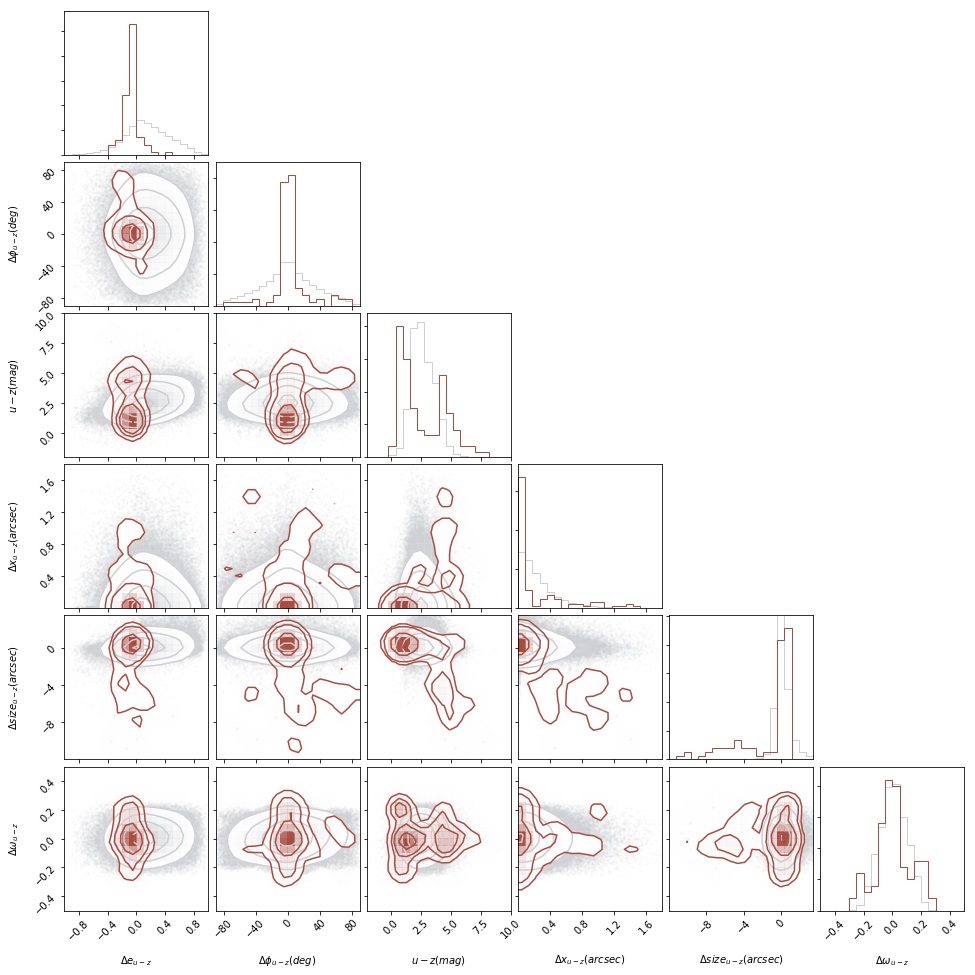
\includegraphics[width=0.9\columnwidth]{cornerplot.png}
\caption{The cornerplot with six features.}
 \label{fig:cornerplot}
\end{figure}
%%%%%%%%%%%%%%%%%%%%%%%%%%%%%%%%%%%%%%

In this figure, we see that the distributions of gray points (SDSS
galaxies) and  red points (OM10 systems) are most significantly
different in the size feature.


\subsection{Machine Classification}
\label{subsec:classification}

We have \FIXME{2323}\footnote{There are 2234 \Object's in the toy object
catalog, not 2323. What's going on here?} realized OM10 lensed systems,
and 16000 SDSS galaxies. In order to make a balanced data set, we
randomly selected an equal number of SDSS galaxies. We shuffled the
order of those two samples so that there will be a roughly same number
of each OM10 and SDSS samples in both the test and the training data,
and, using the \sklearn \texttt{train\_test\_split} method, selected
75\% of the data to be the training set and performed the test on the
remaining 25\%.

According to \sklearn's
\href{http://scikit-learn.org/stable/tutorial/machine_learning_map/index.html}
{flowchart for choosing the right estimator}, we identified three
different algorithms for the classification. We did have more than 50
samples, we were predicting a category, we did have a labeled data, and
we had less than 100K samples in a text data. This yields Linear SVC,
KNeighbors Classifier, and Ensemble classifiers such as Random Forest.
\autoref{fig:roc} shows a receiver operating characteristic (ROC) curve
comparison of these algorithms' performance.

Random forest showed the best performance among the three different
algorithms. The greater the number of estimators, the better the
algorithm performed. For the best algorithm, we were able to achieve a
true positive rate~(TPR) of~98$\%$ and a false positive rate~(FPR)
of~0.04$\%$.

Even though we have high accuracy, because we expect to have much more
non-lensed systems than the lensed systems, we will have more
contaminants in the truly-classified lensed systems than the actual
lensed systems. For instance, we expect to find 10,000 times more
non-lensed systems than the lensed ones. Thus, with 98\% of the TPR and
~0.042\% of the FPR, we will have $\sim430$ contaminants for every truly
classified lensed system. This would translate to about 1 million LSST
candidates for 3000 LSST lensed quasars.

%%%%%%%%%%%%%%%%%%%%%%%%%%%%%%%%%%%%
\begin{figure}
    \centering
    \begin{minipage}{0.48\linewidth}        %% or \columnwidth
        \centering
        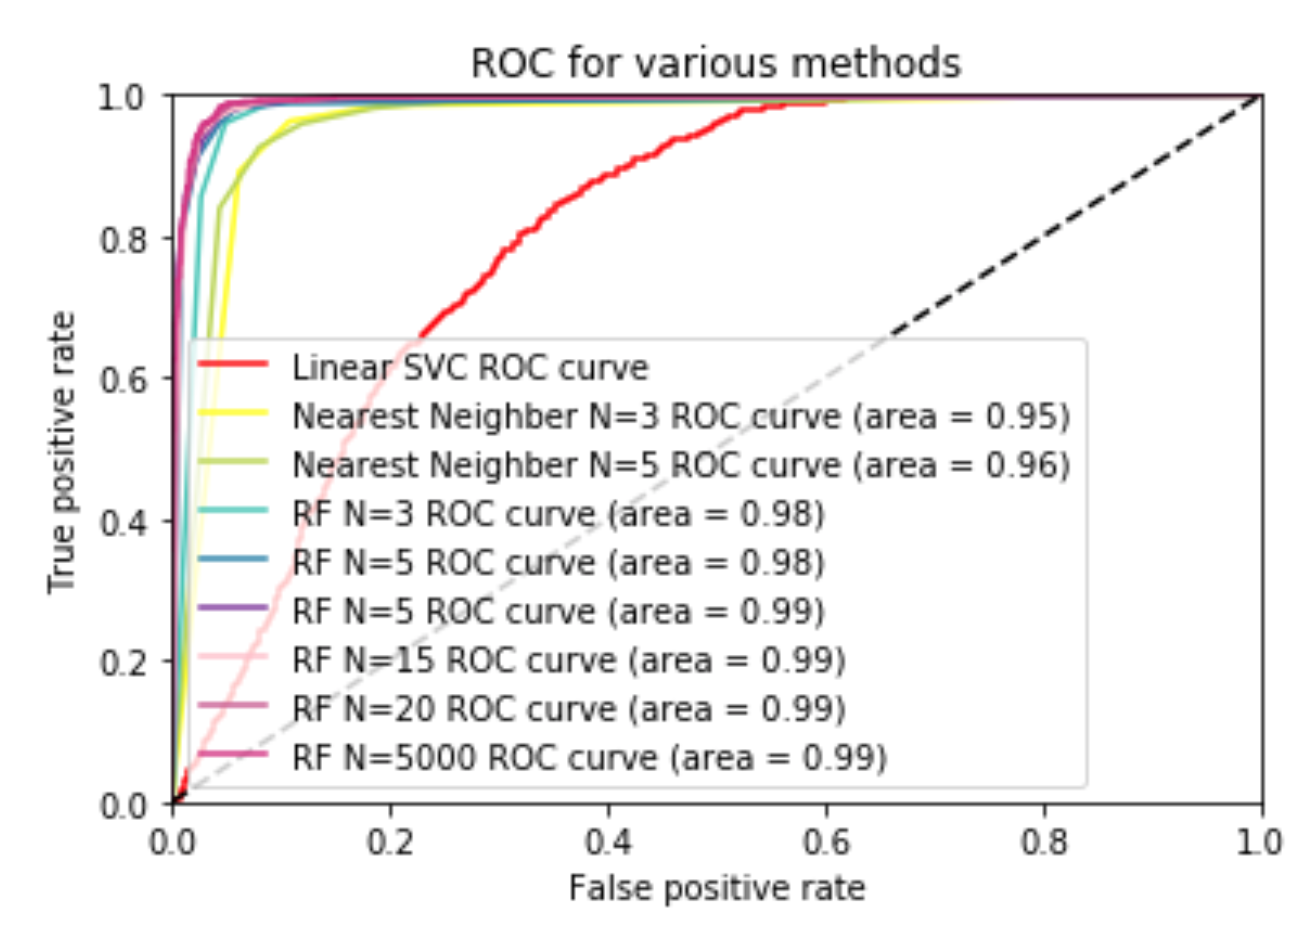
\includegraphics[width=\linewidth]{ML_notmagnified.png}
    \end{minipage}\hfill
    \begin{minipage}{0.48\linewidth}        %% or \columnwidth
        \centering
        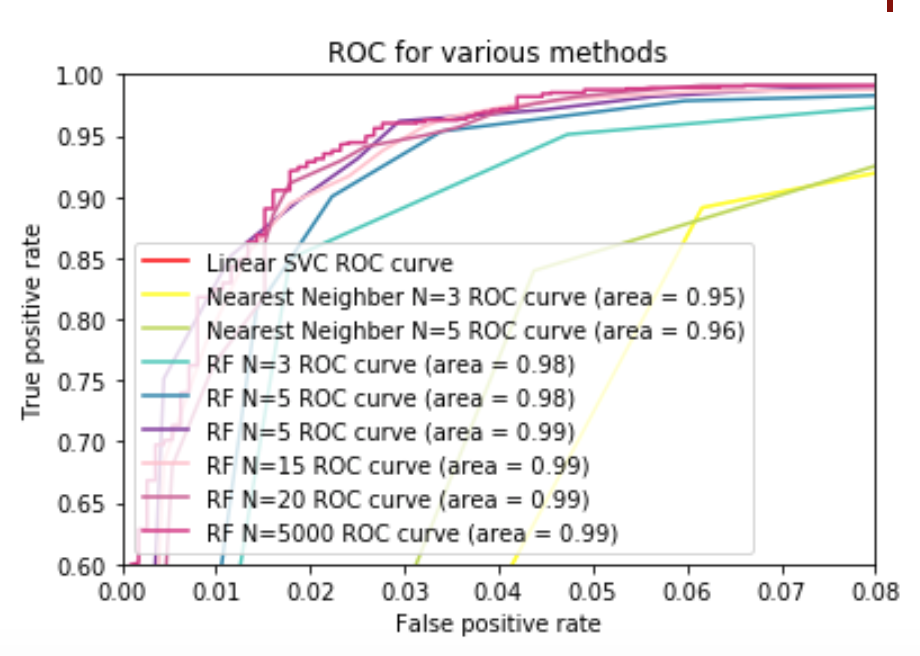
\includegraphics[width=\linewidth]{ML_magnified.png}
         \label{fig:ML Magnified}
    \end{minipage}
    \caption{ROC curves for lens-or-not machine classification on \SLRealizer-emulated LSST \Object data. Left: full view. Right: zoomed-in view over the axes ranges FPR=[0:0.08] and TPR=[0.6:1.0].}
    \label{fig:roc}
\end{figure}
%%%%%%%%%%%%%%%%%%%%%%%%%%%%%%%%%%%%

We can also use the trained Random Forest classifier to quantify the
importance of the input features. We find that, as seen in
\autoref{fig:cornerplot}, the size feature contains the most information
about the \Object classification.  A bar chart of the feature
importances is given in \autoref{fig:featureimportance}.

%%%%%%%%%%%%%%%%%%%%%%%%%%%%%%%%%%%%
\begin{figure}[!h]
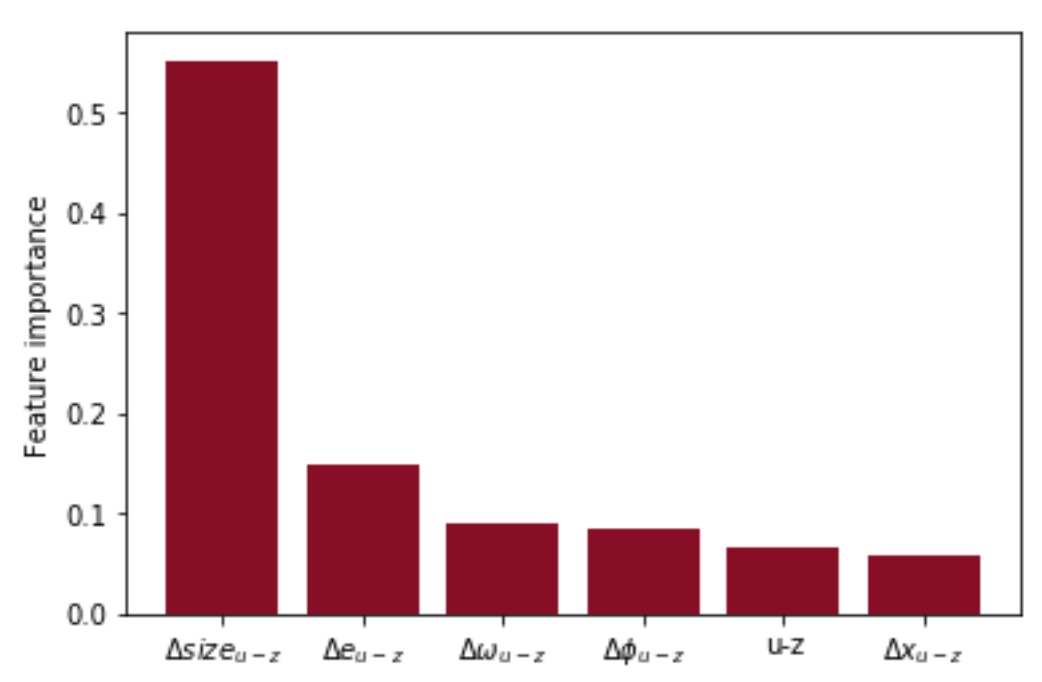
\includegraphics[width=0.4\columnwidth]{FeatureImportance.png}
\caption{Feature importance calculated with the Random Forest algorithm.}
 \label{fig:featureimportance}
\end{figure}
%%%%%%%%%%%%%%%%%%%%%%%%%%%%%%%%%%%%


% ----------------------------------------------------------------------

\section{Discussion and Conclusions}
\label{sec:conclusions}

We implemented a simple model for realizing mock lensed quasar systems,
and used it to emulate a small set of LSST \Object and \Source
measurements, assuming that the LSST deblender cannot resolve the
individual components of the lens systems. We then investigated some
off-the-shelf machine learning classifiers with this simulated data,
finding that the differences in \Object brightness, position,
ellipticity and in particular size between the $u$ and $z$ bands do seem
to enable discrimination between lensed quasars and bright galaxies,
albeit it at sub-percent purity.

We draw the following conclusions, and use them to provide pointers to further work:
\begin{itemize}

    \item \SLRealizer provides a framework for emulating LSST
    measurements of lensed quasar systems. Its initial model assumptions
    are simplistic but these can be refined; most importantly, the
    \SLRealizer model needs to be validated against a set of LSST
    catalogs generated by the DM stack. In the first instance, this
    could be done using the OM10 lenses simulated in DC2.

    \item The difference in observed \Object size between the $u$ and
    $z$ bands contains information useful for lens classification. The
    differences in ellipticity and centroid position are also
    informative, but less so.

    \item Predicting purity requires a realistic non-lens population as
    well as a realistic lens population: further work should include
    refinement of the non-lens population model, and investigation of
    specific problem cases such as physical quasar pairs, star-galaxy
    alignments, star clusters, and so on.

    \item For cosmology, gravitationally lensed systems
    with four images (quads) are more useful than systems with
    two images (doubles). We have not yet looked at the relative classification performance for quads and doubles, but we should.

    \item The time domain should contain much more information about the
    lens classification: further work should include extending
    \SLRealizer to include emulation of the \DIASource and \DIAObject
    tables, and consideration of the time series of all relevant
    features. Since we will have measurements of the image quality and photometric depth for each visit, we will be able to (and will need to) fold this information in as well.

    \item Feature extraction could be improved through fitting a
    physical lens model to the catalog data. This could be done by
    realizing both a lens model and the catalog measurements onto
    matchin pseudo-image grids and computing a misft statistic, and then
    optimizing the model in the usual way. An alternative approach could
    be to use deep learning networks to bypass the feature extraction
    step, instead just providing all available catalog data,
    suitably-packaged.

    \item If the LSST deblender does separate the components of lensed quasar systems, this should provide significantly more information
    about lens classification. Future work should include emulating the action of such a deblender: this will involve a more complex \Object table, including meaningful ``neighbor'' linkages.

\end{itemize}


% ----------------------------------------------------------------------

\subsection*{Acknowledgments}

% 
This is the text imported from \code{acknowledgments.tex}, and will be replaced by some standard LSST DESC boilerplate at some point.
% 


Author contributions are listed below. \\
Jenny Kim: Initial algorithm and code development, wrote paper. \\
Ji Won Park: Improved algorithm and code development, edited paper. \\
Phil~Marshall: Initiated  project, advised on motivation, model construction and testing. \\
Mike~Baumer: Advised on LSST data characteristics, model construction and testing. \\
Steve~Kahn: Advised on LSST data characteristics, model construction and testing. \\
Rahul~Biswas: Advised on LSST observing cadence, catalog characteristics, error model. \\


%{\it Facilities:} \facility{LSST}
% Include both collaboration papers and external citations:
\bibliography{desc-tex/bib/lsstdesc,../slrealizer}

\end{document}
% ======================================================================
%
